This part defines the development of the tool chain itself. It defines
the steps to achieve for the implementation of the tool chain.

%----------------------
\subsection{OpenETCS Tool chain lifecycle}
The tool chain lifecycle is depicted figure  \ref{fig:TC_lifecycle}.

\begin{figure}[ tbp]
\centering
  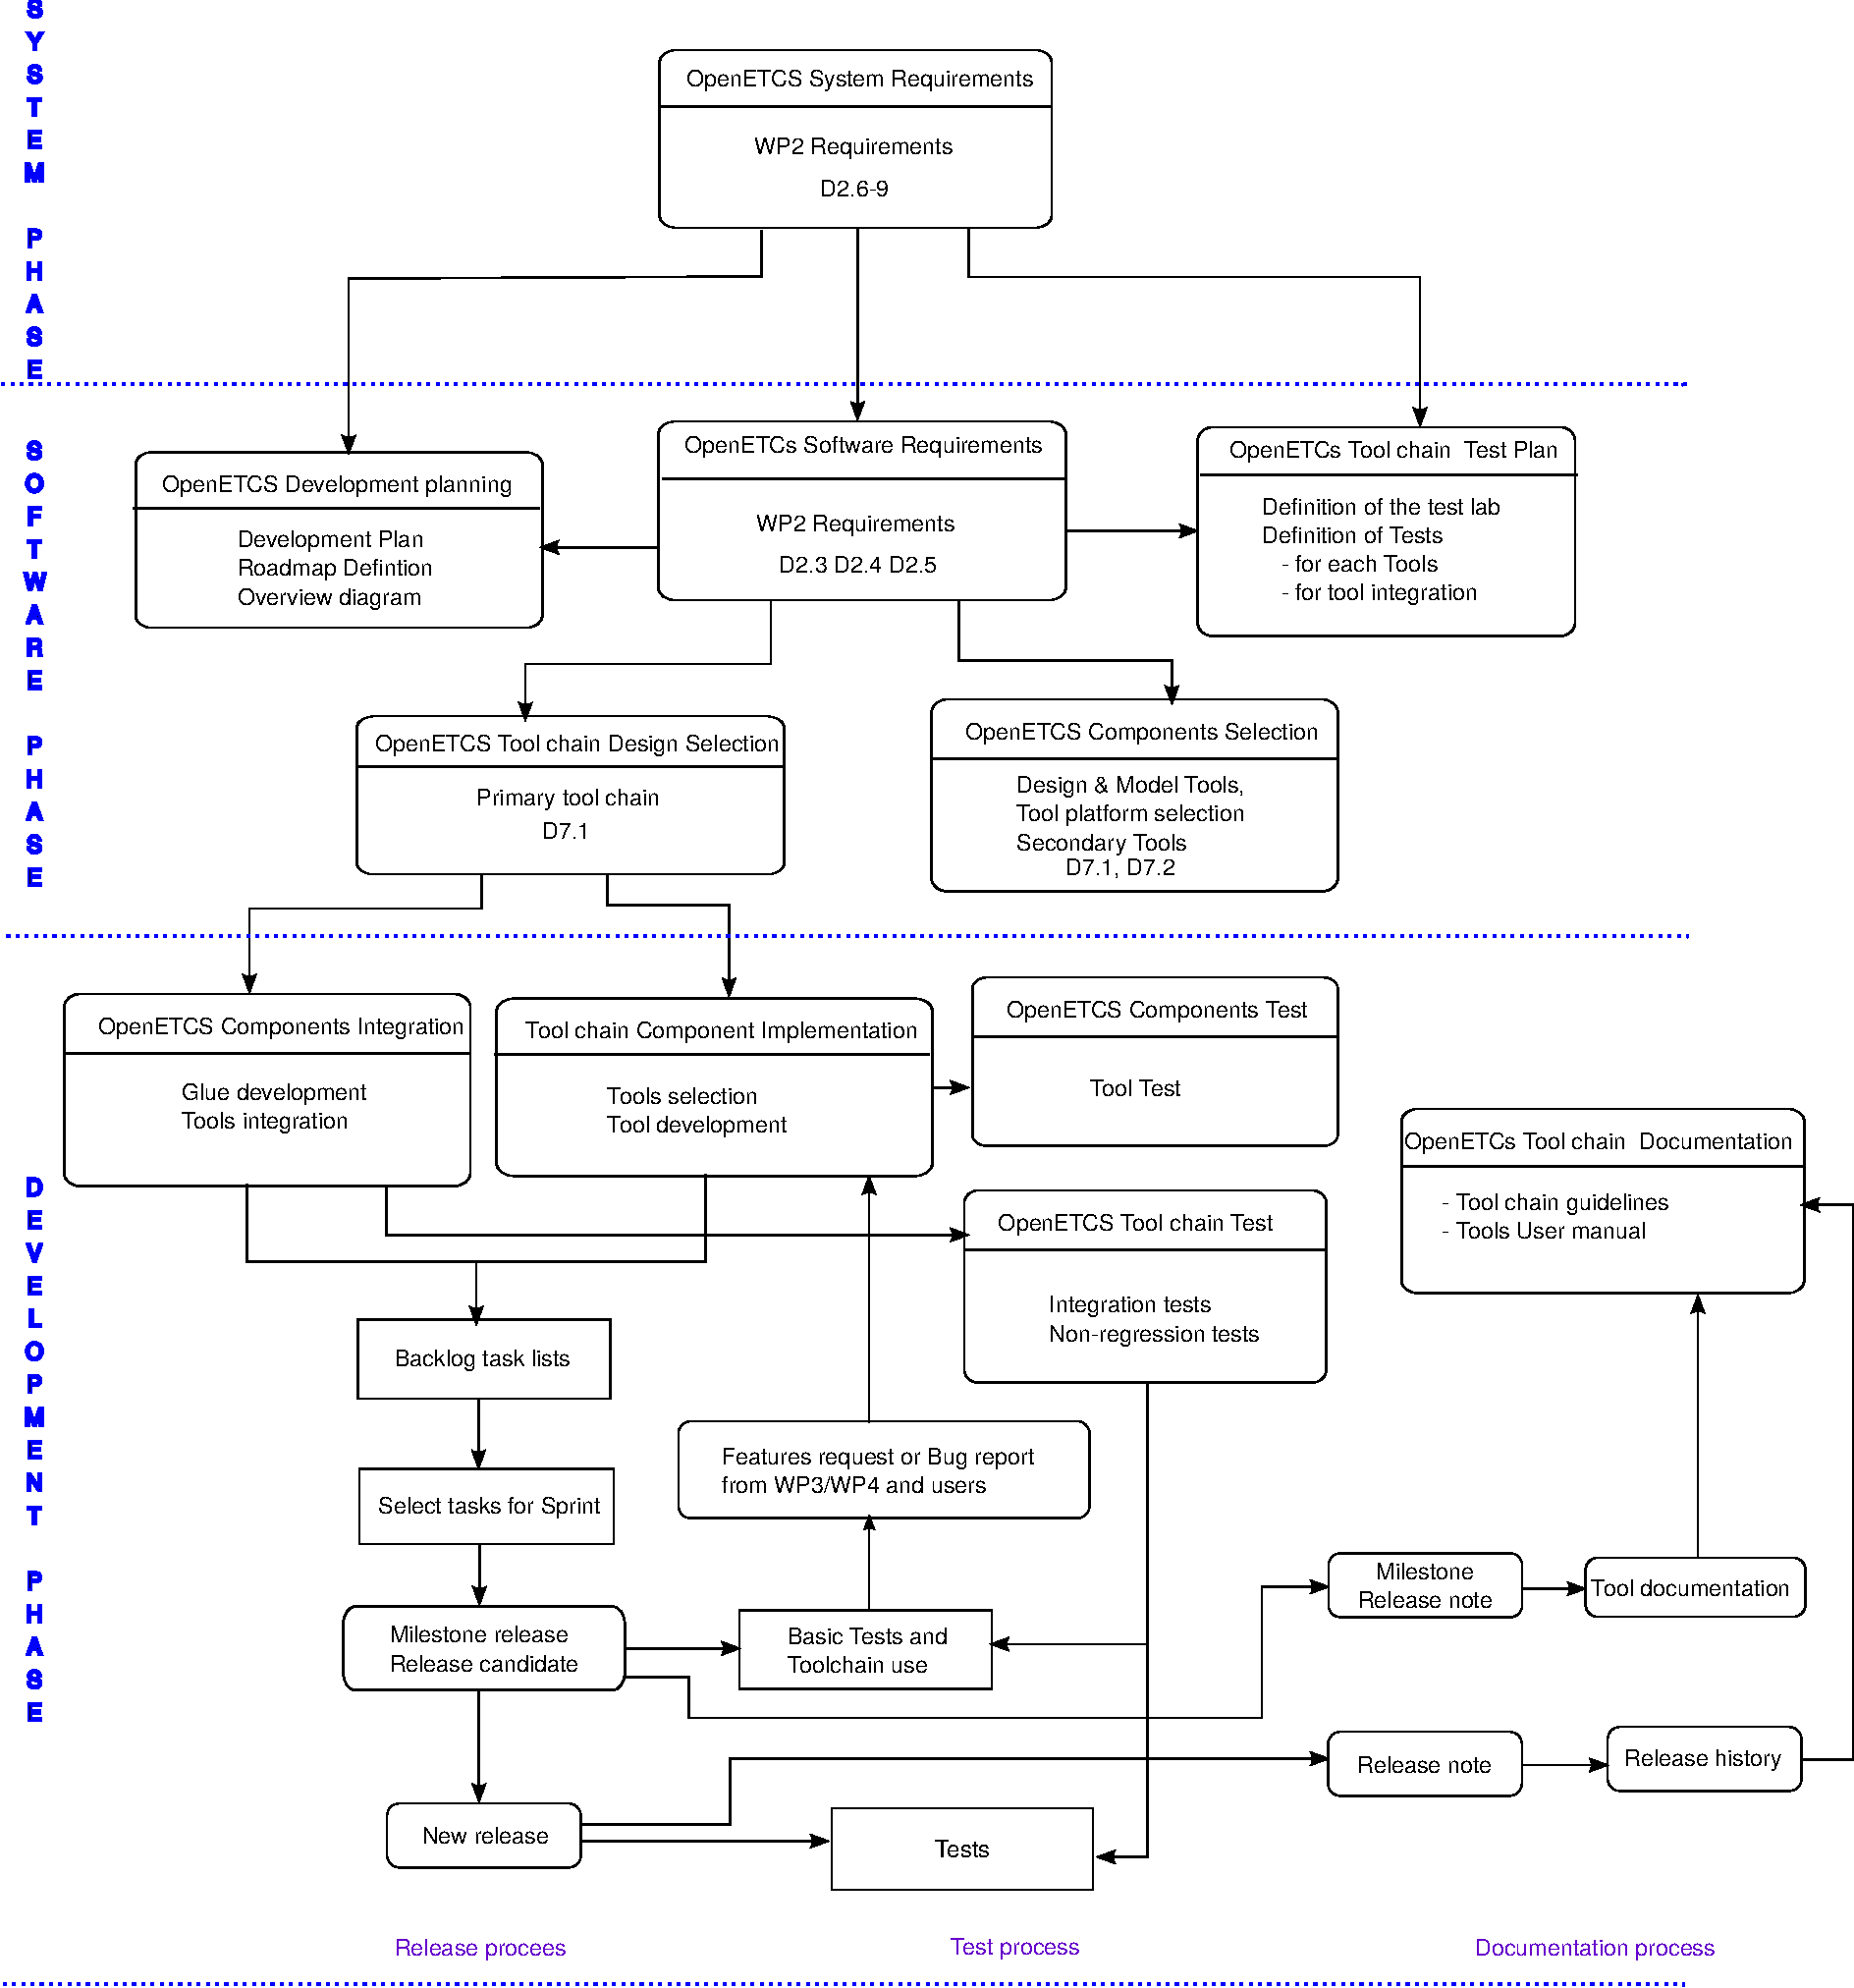
\includegraphics[width= \textwidth]{toolchain_lifecycle}
  \caption{The OpenETCS tool chain life cycle}
  \label{fig:TC_lifecycle}
\end{figure}

\subsection{OpenETCS Tool chain use of \gls{COTS}}
To design the life cycle defined in the previous section, the tool chain will
use the components selected by the WP7.  The tool chain will intensively use 
\gls{COTS} application to reduce   the cost for the development of the
\gls{OBU}.

The decision on the selection of means of description, tools and tool platform
are defined in the document \cite{D7.1}. The selection of the secondary tools,
e.g. the choice of verification and validation tools are described in \cite{D7.2}.

\subsection{OpenETCS Tool chain development}
The tool chain development will follow the SCRUM process.
The following activities will be covered  by the tool chain development.
\begin{itemize}
\item openETCS tool chain architecture specification\\
Definition of the tool chain composition (covers by T7.1 \cite{D7.1}
and T7.2 \cite{D7.2})
\item openETCS tool chain design specification \\
Definition of how the tool chain is implemented including the
definition of the interoperability mechanism
\item Software development\\
Implementation of the tool chain in particular for the need of tool interoperability
\item Test and verification plan\\
Definition of how to test the tool chain.
\item Agile software development guidelines\\
Guidelines on how to use the tool chain in an agile development.
\end{itemize}

The tool chain specification is out of the scope of the document. It
has been defined by the WP2, the requirements are listed in Appendix \ref{app:wp2req}.
 	

%%% Local Variables:
%%% TeX-master: "WP7-ToolChainDevelpmentPlan"
%%% End:
